\documentclass[nonacm]{acmart}

%%
%% \BibTeX command to typeset BibTeX logo in the docs
\AtBeginDocument{%
  \providecommand\BibTeX{{%
    \normalfont B\kern-0.5em{\scshape i\kern-0.25em b}\kern-0.8em\TeX}}}

%%
%% These commands are for a JOURNAL article.
%% PLEASE IGNORE THEM!
\acmJournal{TOIT}
\acmVolume{37}
\acmNumber{4}
\acmArticle{111}
\acmMonth{8}

%%
%% end of the preamble, start of the body of the document source.
\usepackage{textcomp}
\usepackage{multirow}
\usepackage{array}
\usepackage{hyperref}
\usepackage{enumitem}
\usepackage{listings}
\lstset{
  basicstyle=\ttfamily\small,
  breaklines=true,
  columns=fullflexible
}

% TikZ and plotting packages
\usepackage{tikz}
\usepackage{pgfplots}
\pgfplotsset{compat=1.18}
\usetikzlibrary{patterns,arrows.meta}

\newcolumntype{M}[1]{>{\centering\arraybackslash}m{#1}}
%Definition of Colors - Start
\definecolor{xred}{RGB}{255,0,0}
\definecolor{xblue}{RGB}{68,114,196}
\definecolor{xgreen}{RGB}{0,176,80}
\definecolor{xpurple}{RGB}{112,48,160}
\definecolor{xorange}{RGB}{237,125,49}
%Definition of Colors - End

\setcopyright{none}
\settopmatter{printacmref=false} % Removes citation information below abstract
\renewcommand\footnotetextcopyrightpermission[1]{} % removes footnote with conference information in first column
\pagestyle{plain}
\begin{document}

\title{Development of a Power Consumption Dashboard for On-Premises Servers of Small and Medium-Sized Enterprises}
\input{section/authors}
%Je nach dem in welcher Sprache ihr euer Paper schreiben wollt, benutzt bitte entweder den Deutschen-Titel oder den Englischen (einfach aus- bzw. einkommentieren mittels '%')

\begin{abstract}
%Deutsch
%\textbf{ABSTRACT}

%Englisch
\textbf{ABSTRACT}
Rising energy costs pose significant challenges for small and medium-sized enterprises (SMEs) 
operating on-premise server infrastructures. This paper presents a scalable, serverless energy
monitoring system that integrates Internet of Things (IoT) power monitoring, smart meter data,
and real-time electricity market pricing. Built on Amazon Web Services (AWS), the system combines 
data from Sagemcom smart meters and NOUS A5T PowerCable devices with European Power Exchange (EPEX) 
Spot market prices to enable cost-aware workload management. Comprehensive energy profiling across 
diverse operational scenarios demonstrates that intelligent workload scheduling based on electricity 
pricing can reduce operational costs by up to 10.50 cent/kWh in our test intervall for the 
CPU stress test (peak load). A 24-hour evaluation period revealed distinct power consumption patterns, 
ranging from 172.2W (idle) to 662.25W (peak load). A practical implementation framework and empirical 
evidence supporting the economic viability of energy-aware server management for SMEs are provided.
\end{abstract}

\maketitle

%Je nach dem in welcher Sprache ihr euer Paper schreiben wollt, benutzt bitte entweder den Deutschen-Titel oder den Englischen (einfach aus- bzw. einkommentieren mittels '%')

\section{Introduction}
\label{introduction:introduction}
The rapid escalation of energy prices has emerged as a significant operational challenge for small and medium-sized enterprises (SMEs), particularly those maintaining on-premise server infrastructures. As electricity costs become an increasingly substantial component of IT expenditures, optimizing energy efficiency and cost management is critical for ensuring business sustainability and competitiveness \cite{ec2022energyefficiencysmes}. Server operations, which are indispensable for business continuity, exhibit highly variable energy consumption depending on workload intensity, maintenance activities, and system states.

Despite the importance of energy-aware management, most SMEs lack transparency regarding the power consumption profiles of their server activities. Routine tasks such as reboots, backups, software updates, and maintenance can each have distinct energy footprints, yet their impact on overall operational costs often remains opaque. This lack of actionable insight hinders the ability of SMEs to strategically schedule energy-intensive operations, especially in the context of dynamic electricity pricing \cite{ristic2021iotenergymanagement}.

A parallel can be drawn to the management of photovoltaic (PV) systems, where owners are advised to operate high-consumption appliances during periods of peak solar generation. Similarly, SMEs could benefit from aligning server workloads with periods of lower electricity prices or increased renewable energy availability, thereby reducing costs and supporting sustainability objectives.

The detailed system architecture and methodological approach are described in Section~\ref{methodology:methodological-approach}. Empirical results and analysis are presented in Section~\ref{results:results}.

This gap is addressed by proposing a comprehensive, serverless architecture that integrates smart meter data, Internet of Things (IoT)-based server power monitoring, and real-time electricity market pricing into a unified, cloud-based dashboard.

The primary objectives of this research are as follows:
\begin{itemize}
\item To develop a scalable system for collecting and analyzing detailed energy consumption data from SME server infrastructures
\item To enable real-time correlation of server activities with electricity market prices to inform cost-effective workload scheduling
\item To demonstrate the practical benefits of the proposed approach through empirical evaluation across diverse operational scenarios
\end{itemize}

To achieve these aims, Amazon Web Services (AWS) serverless technologies, including API Gateway, IoT Core, Lambda, and DynamoDB, are leveraged to collect and process data from Sagemcom smart meters and NOUS A5T PowerCable devices. Visualization and analysis are facilitated through Amazon QuickSight, while real-time electricity prices from the European Power Exchange (EPEX) Spot market are integrated via the smartENERGY API (see Appendix~\ref{appendix:strompreis-api}). The complete implementation, including source code and deployment instructions, is made available in a public repository (see Appendix~\ref{appendix:github-docs}).

The remainder of this paper is organized as follows: Section~\ref{related_work:related-work} reviews related work in energy management and optimization, Section~\ref{methodology:methodological-approach} details the system architecture and methodology, Section~\ref{results:results} presents our experimental findings and cost analysis, Section~\ref{conclusion:conclusion} concludes with future research directions, and Section~\ref{references:references} provides references. Detailed API specifications and implementation guides are provided in the appendices.
%Je nach dem in welcher Sprache ihr euer Paper schreiben wollt, benutzt bitte entweder den Deutschen-Titel oder den Englischen (einfach aus- bzw. einkommentieren mittels '%')

%Deutsch
%\section{Stand des Wissens}

% Englisch
\section{Related Work}
\label{related_work:related-work}
A growing body of research addresses the challenges of energy measurement, management, and optimization in server and data center environments. This section reviews key contributions in four thematic areas: (1) process-level energy measurement, (2) data center management approaches, (3) IoT and building management systems, and (4) policy context and foundations. A synthesis of the research gap and the unique contribution of this work is provided. The proposed solution is detailed in Section~\ref{methodology:methodological-approach}, and a comparison of results with prior work is discussed in Section~\ref{results:results}.
\paragraph{\textbf{Process-Level Energy Measurement:}}
Recent advances have enabled more granular attribution of energy consumption within server environments. Qiao et al. (2023) introduced Wattmeter, a Linux-level tool that attributes energy usage to individual processes and informs CPU scheduling decisions. While this approach is valuable for operating system research, it does not integrate electricity pricing or provide visualization capabilities, limiting its applicability for cost-aware management \cite{qiao2023wattmeter}. Similarly, Zhang et al. (2022) developed a method for container-level energy attribution in microservice architectures, but did not address real-time market price integration. Khan and Varghese (2021) proposed energy-aware scheduling algorithms for heterogeneous server clusters, focusing on power consumption patterns without considering dynamic electricity pricing \cite{zhang2022container,khan2021energy}.
\paragraph{\textbf{Data Center Management Approaches:}}
Energy optimization in data centers has been approached from multiple perspectives. Chen et al. (2022) applied machine learning to enable cost-aware demand response, achieving significant peak-shaving in large-scale cloud environments. Cheung et al. (2021) proposed linear models correlating CPU utilization with power consumption, offering a simpler alternative for data center operators. Smith et al. (2023) analyzed the trade-offs between cost and carbon emissions, highlighting the complexity of multi-objective optimization. Mahmoud et al. (2020) combined workload prediction with renewable energy forecasts for hybrid optimization, while Wang et al. (2023) employed reinforcement learning to dynamically allocate resources in response to variable electricity prices \cite{chen2022datacentermodel,cheung2021utilizationmodel,smith2023warofefficiencies,mahmoud2020cost,wang2023reinforcement}.
\paragraph{\textbf{IoT and Building Management Systems:}}
The integration of IoT technologies has expanded the scope of energy management beyond traditional data centers. Gholami et al. (2020) provided a comprehensive survey of smart building energy management systems, emphasizing IoT architectures and analytics. Ristić et al. (2021) designed an IoT-based energy management platform specifically for SMEs, demonstrating the potential for tailored solutions in smaller organizations. Palacios-Garcia et al. (2022) explored edge computing for real-time energy management in distributed environments, while Kumar et al. (2021) introduced blockchain-enabled frameworks for secure energy data sharing. Lopez-Garcia et al. (2023) proposed standardized APIs to enhance interoperability among energy management systems \cite{gholami2020energymanagement,ristic2021iotenergymanagement,palacios2022edge,kumar2021blockchain,lopez2023standardized}.
\paragraph{\textbf{Policy Context and Foundations:}}
Policy and regulatory frameworks play a critical role in shaping energy management practices. The International Energy Agency (2023) provides high-level policy guidance for data centers, and the European Commission (2022) has compiled case studies highlighting successful energy efficiency initiatives in SMEs. Siano (2014) established foundational concepts for demand-response programs, while Ahmad et al. (2021) analyzed regulatory frameworks affecting SME energy management across jurisdictions. The Green Grid Association (2021) introduced advanced metrics for assessing data center sustainability, and Koomey and Masanet (2021) provided updated global estimates of data center energy consumption, underscoring the importance of server-level optimizations \cite{iea2023datacenters,ec2022energyefficiencysmes,siano2014demandresponse,ahmad2021regulatory,greengrid2021beyond,koomey2021does}.
\paragraph{\textbf{Gap Analysis and Contribution:}}
Despite significant progress in each of these domains, existing solutions typically address only isolated aspects of the broader challenge. To the best of our knowledge, no prior work offers a holistic system that combines per-process energy attribution in SME servers, smart meter data integration, real-time electricity price correlation, and a unified dashboard for actionable insights. This gap is addressed by proposing an AWS-based architecture (Section~\ref{methodology:prototype}) that unifies kernel-level process metering, smart meter feeds (Appendix~\ref{appendix:energylive-api}), and market price polling (Appendix~\ref{appendix:strompreis-api}) into a comprehensive visualization and decision-support platform. The complete implementation details and source code are available in a public repository (Appendix~\ref{appendix:github-docs}), enabling reproducibility and further research in this domain.
%Je nach dem in welcher Sprache ihr euer Paper schreiben wollt,
%benutzt bitte entweder den Deutschen-Titel oder den Englischen (einfach aus- bzw. einkommentieren mittels '%')

%Deutsch
%\section{Methodischer Ansatz}

%Englisch
\section{Methodological Approach}
\label{methodology:methodological-approach}
This section outlines the methodological approach taken to design, implement, and evaluate an energy-aware server management solution for small and medium-sized enterprises (SMEs).
It describes the overall use case, the technical architecture of the prototype, and the integration of real-time energy consumption and electricity price data.

\subsection{Use Case Description}
\label{methodology:use-case-description}
The use case centers on an SME operating on-premise server infrastructure, seeking to optimize energy consumption and costs amid rising electricity prices. Key stakeholders include the SME IT administrator, who manages server operations and energy monitoring, and external data providers such as smart meters and electricity market APIs. The system aims to enable the administrator to schedule energy-intensive tasks during periods of lower electricity prices, thereby minimizing costs and supporting sustainability goals.
\begin{figure}[h!]
\centering
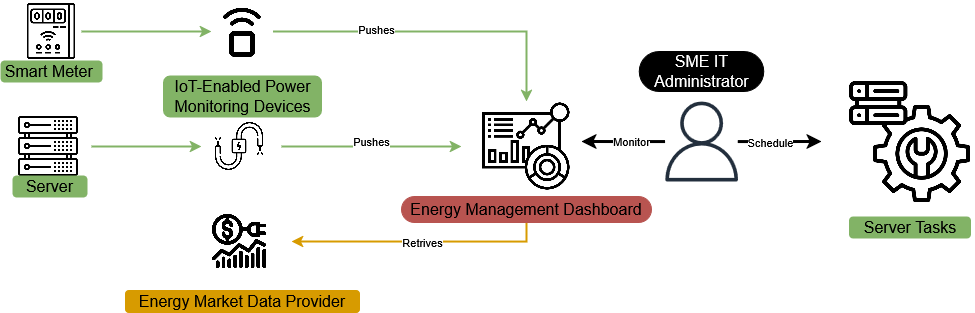
\includegraphics[width=0.8\textwidth]{fig/high_level_use_case.png}
\caption{Overall use case of server administrator utilizing the energy management dashboard.}
\label{fig:highleveluse}
\end{figure}
As illustrated in Figure~\ref{fig:highleveluse}, energy consumption data is continuously collected from both facility-level smart meters and device-level IoT power monitors. Simultaneously, real-time electricity prices are retrieved from market data providers (e.g., EPEX Spot). These data streams are integrated and visualized via a cloud-based dashboard, providing actionable insights and recommendations for workload scheduling.
\newpage
\subsection{Prototype}
\label{methodology:prototype}
The prototype implements a cloud-native architecture leveraging Amazon Web Services (AWS) to ensure scalability, reliability, and cost-effectiveness—key considerations for SMEs with limited IT resources. Figure~\ref{fig:architecture} illustrates the system architecture. The complete implementation details, including infrastructure as code and configuration files, are available in the project materials and are further described in Appendix~\ref{appendix:github-docs}.
\begin{figure}[htbp]
\centering
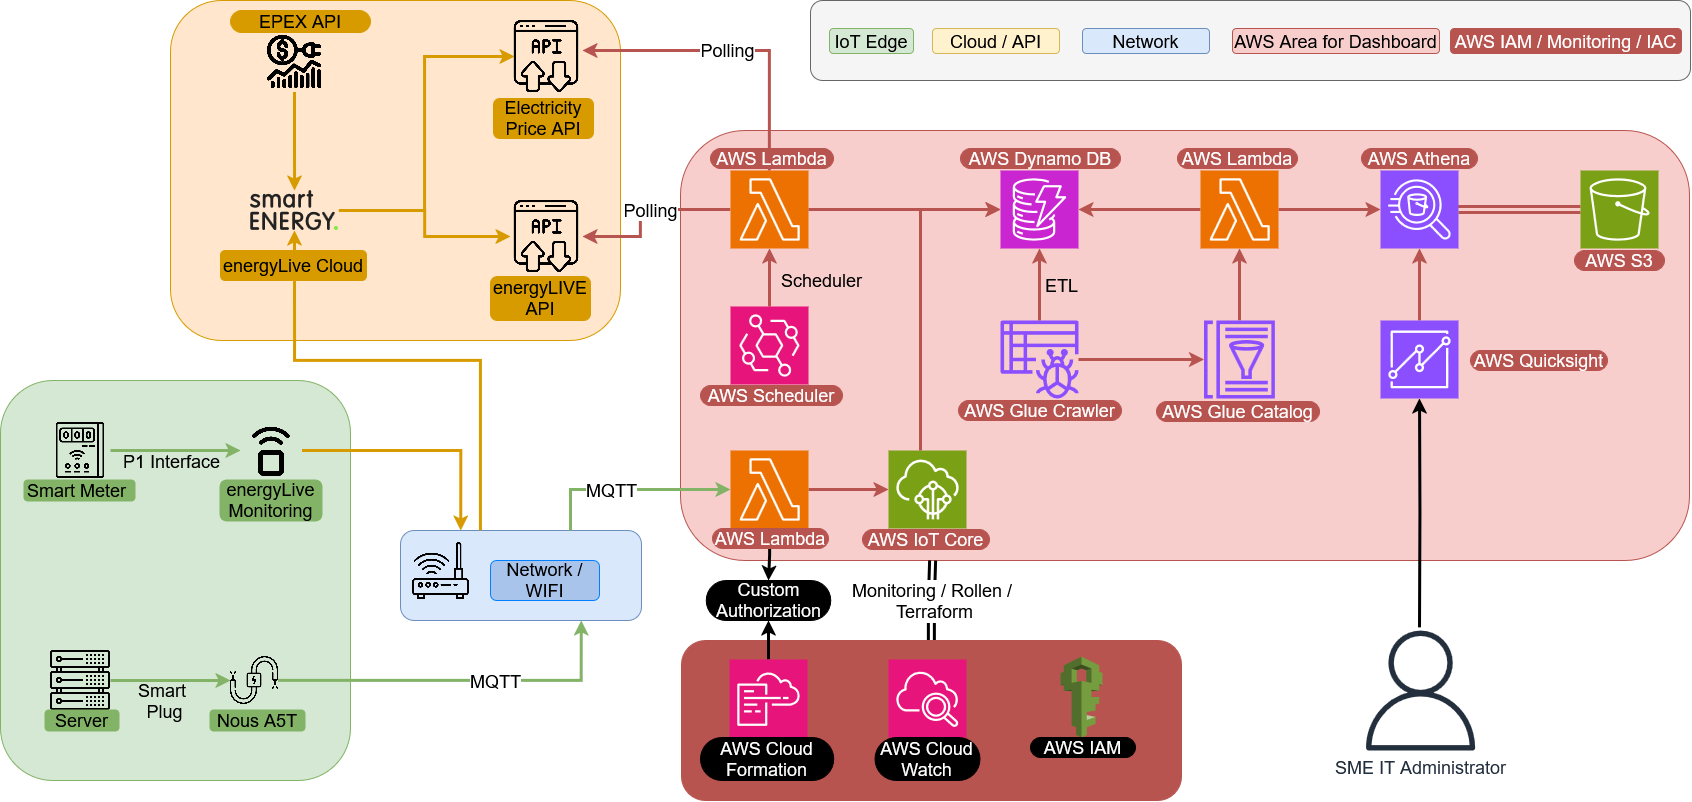
\includegraphics[width=1.1\textwidth]{fig/architektur_new_2.png}
\caption{System Architecture of the AWS implementation.}
\label{fig:architecture}
\end{figure}
At the edge, a smart meter with a P1 interface and a NOUS A5T smart plug\footnote{See Appendix~\ref{appendix:tasmota-config} for configuration details.} are deployed within the SME's local network. The smart meter provides aggregate facility-level data, while the NOUS A5T delivers device-specific power usage via MQTT. Data is ingested into the cloud using a hybrid of polling (for smart meter and market prices) and message-based (for IoT devices) mechanisms.
AWS Lambda functions, triggered by scheduled polling or MQTT messages, process incoming data. AWS IoT Core manages secure MQTT communication, while API Gateway and Lambda handle RESTful interactions with external APIs. All data is stored in AWS DynamoDB for low-latency access. AWS Glue and Athena enable automated data cataloging and ad hoc querying, respectively. Visualization is provided through AWS QuickSight dashboards, allowing administrators to correlate energy usage with market prices and identify optimization opportunities. Infrastructure is provisioned using AWS CloudFormation for reproducibility, and security is enforced via AWS IAM and CloudWatch.
\subsection{Evaluation Approach}
\label{methodology:evaluation-approach}
To evaluate the effectiveness of the approach, a comprehensive evaluation strategy is implemented that addresses technical performance, server energy consumption patterns, and economic impacts. This multi-faceted evaluation provides insights into both the system's technical capabilities and its practical utility for SME operators. The results of these experiments are presented in Section~\ref{results:results}.

Server energy consumption analysis forms the core of the measurement approach. Using the NOUS A5T PowerCable device, detailed measurements of a single server under various operational scenarios are conducted to establish energy consumption profiles. Specifically, the following workloads (WL) are examined:

\begin{enumerate}[label=WL\arabic*]
    \item \textbf{Maximum computational load:} Simulation of 100\% CPU utilization across all
    cores using the stress-ng tool on a Linux virtual machine. The stress-ng
    command will be configured to spawn CPU-intensive worker processes equal to
    the number of available virtual CPUs, ensuring maximum load across all cores.
    This scenario represents peak computational demand typical of batch processing
    or intensive data analysis tasks. \cite{stressng2020}

    \item \textbf{I/O stress testing:} This WL conduct I/O stress testing to evaluate
    power consumption during intensive disk operations. Using fio (Flexible I/O Tester),
    we will simulate maximum Solid State Drive (SSD) utilization with sequential and random read/write
    patterns. This I/O-intensive scenario represents workloads common in database operations,
    log processing, and large file transfers, providing insights into storage
    subsystem energy requirements under heavy load.

    \item \textbf{System reboot cycle:} Measurement of the overall power consumption profile
    during a full reboot sequence of the host machine, capturing the energy
    requirements during shutdown, boot, and system initialization phases. This
    provides insights into the energy costs associated with maintenance operations
    and system updates.

    \item \textbf{Maintenance operations:} Monitoring of energy consumption during typical
    maintenance activities, specifically the patching process of a Linux virtual
    machine. This scenario represents regular administrative tasks that SMEs must
    perform to maintain security and system integrity.

    \item \textbf{Idle state:} Establishing the baseline energy consumption when the server is
    in an idle state with minimal active processes. This measurement is crucial
    for understanding the fixed energy costs of maintaining server availability
    even during periods of low utilization. \cite{moran2024dissecting,agilewatts2022}
\end{enumerate}

For each WL, the total energy usage consumption is measured in kilowatt-hours (kWh) and power consumption patterns over time, establishing detailed energy profiles that can be correlated with specific operational states. These measurements reveal the energy intensity of different server activities and identify potential optimization opportunities, such as scheduling high-consumption tasks during periods of lower electricity pricing or implementing more efficient idle-state management.

To ensure reliable and representative measurements, each test scenario will be
conducted with specific time windows (TW):

\begin{enumerate}[label=TW\arabic*]
    \item For maximum computational load and I/O stress testing scenarios, each
    test window will span 15 minutes of load and 15 minutes of idle to capture steady-state 
    behavior and account for any thermal effects or performance throttling that may occur during
    sustained high-load operations.

    \item System reboot cycle measurements will be conducted over multiple
    iterations, with each complete cycle (shutdown to fully operational)
    typically lasting 5-10 minutes.

    \item Maintenance operation measurements will cover the entire duration of
    typical update processes, estimated at 5-10 minutes per session, including
    download, installation, and post-update system stabilization periods.

    \item Idle state measurements will be conducted over longer 60-minute windows
    during off-peak hours to establish accurate baseline consumption patterns and
    capture any periodic background system activities.
\end{enumerate}

A minimum cool-down period of 10 minutes has to be assured between test iterations to 
ensure thermal conditions return to baseline.

\subsection{Test Infrastructure Setup}
\label{methodology:test-infrastructure-setup}

To conduct the stress testing scenarios described in WL1 and WL2, a dedicated test infrastructure 
in the form of a Ubuntu 24.04.2 LTS virtual machine was established within a Proxmox virtualization
environment.

\subsubsection{CPU Stress Testing Configuration}
\label{methodology:cpu-stress-testing-configuration}

For maximum computational load testing (WL1), a dedicated stress-ng scheduling 
script was developed to generate sustained CPU load across all available cores. 
The stress-ng tool was selected for its ability to create reproducible, 
high-intensity computational workloads suitable for energy consumption analysis.

The CPU stress testing implementation (see Appendix~\ref{appendix:github-docs} 
for implementation details) includes the following characteristics:
\begin{itemize}
    \item \textbf{Full CPU utilization:} Spawns worker processes equal to the 
    number of available virtual CPUs (56 logical processors)
    \item \textbf{Sustained load patterns:} Maintains 100\% CPU utilization 
    for the entire 15-minute test duration
    \item \textbf{Thermal consideration:} Includes cooling periods between test 
    cycles to prevent thermal throttling effects
    \item \textbf{Automated scheduling:} Uses the \texttt{at} command for 
    precise timing synchronization with energy measurement intervals
    \item \textbf{Comprehensive logging:} Records CPU utilization metrics and 
    timestamps for correlation with power consumption data
\end{itemize}

The stress-ng configuration utilizes the command 
\texttt{stress-ng --cpu 56 --timeout 900s} to ensure maximum computational 
load across all processor cores. This approach simulates intensive batch 
processing workloads typical in SME environments, such as data analysis, 
compilation tasks, or scientific computing operations.

Similar to the I/O stress testing, the CPU stress script supports configurable 
test cycles with alternating 15-minute stress periods and 15-minute idle 
periods, enabling direct comparison of energy consumption between high-load 
and baseline states. The automated cleanup and logging mechanisms ensure 
consistent test conditions and comprehensive data collection for subsequent 
analysis.

\subsubsection{Storage Configuration}
\label{methodology:storage-configuration}
The original virtual machine configuration had insufficient free disk space for intensive
I/O testing that requires substantial temporary file creation. To address this limitation, a
dedicated 50GB virtual disk was provisioned and attached to the test virtual machine as a
secondary storage device.

The additional disk was formatted with the ext4 filesystem providing 50GB of available space
exclusively for I/O testing operations. The disk was configured with I/O threading enabled in 
the Proxmox hypervisor to maximize I/O performance and ensure realistic energy consumption
measurements under high-load conditions.
This configuration ensures that:

\begin{itemize}
    \item I/O testing operations do not interfere with system operations on the primary disk
    \item Sufficient space is available for creating large test files (up to 32GB total)
    \item Test data can be isolated and cleaned up after each measurement cycle
    \item Storage performance characteristics can be measured independently
\end{itemize}


\subsubsection{Automated Test Scheduling}
\label{methodology:automated-test-scheduling}
To ensure precise timing alignment with the 15-minute measurement intervals of the energy
monitoring system, automated test scheduling scripts were developed using the \texttt{at}
command scheduler. The FIO stress testing implementation (see Appendix~\ref{appendix:github-docs} 
for implementation details) includes the following characteristics:


\begin{itemize}
    \item \textbf{Configurable test cycles:} Support for multiple 15-minute I/O stress periods
    followed by 15-minute idle periods
    \item \textbf{Maximum I/O load generation:} Utilizes 4 parallel FIO jobs with 32-depth I/O queues,
    mixed random read/write patterns (70\% read, 30\% write), and variable block sizes (4KB to 1MB)
    \item \textbf{Direct I/O operations:} Bypasses operating system caches to ensure actual disk I/O
    and realistic power consumption
    \item \textbf{Automatic cleanup:} Removes test files after each cycle to prevent disk space
    exhaustion
    \item \textbf{Comprehensive logging:} Records detailed performance metrics and timestamps
    for correlation with energy measurements
\end{itemize}

This automated approach ensures that I/O stress testing can be precisely 
synchronized with energy measurement intervals, enabling accurate correlation 
between storage workload intensity and power consumption patterns.
%Je nach dem in welcher Sprache ihr euer Paper schreiben wollt,
%benutzt bitte entweder den Deutschen-Titel oder den Englischen (einfach aus- bzw. 
%einkommentieren mittels '%')

%Deutsch
%\section{Ergebnisse}

%Englisch
\section{Results}
\label{results:results}
This section presents the key findings from our energy-aware server management system evaluation, 
focusing on system implementation outcomes and quantitative energy consumption analysis. 
The complete analysis scripts and raw data are available in our public repository 
(see Appendix~\ref{appendix:github-docs}).

The methodology used to obtain these results is described in Section ~\ref{methodology:methodological-approach}.
These findings support the conclusions drawn in Section~\ref{conclusion:conclusion}.

\subsection{System Implementation}
\label{results:system-implementation}
The prototype system was successfully deployed on AWS infrastructure using Infrastructure as Code 
principles, with all configuration files and deployment scripts available in the repository 
(see Appendix~\ref{appendix:github-docs}). Key technical achievements include:

\begin{itemize}[noitemsep,topsep=0pt]
    \item Real-time data ingestion with sub-second latency from NOUS A5T smart plugs via MQTT
    \item Reliable 1-minute interval data collection from energyLive API (see Appendix~\ref{appendix:energylive-api}) 
    \item Reliable 15-minute interval data collection from EPEX Spot API (see Appendix~\ref{appendix:strompreis-api})

    \item Scalable DynamoDB storage with consistent sub-10ms query response times
\end{itemize}

\subsection{Energy Consumption Analysis}
\label{results:energy-analysis}
Our analysis revealed distinct power consumption patterns across different workload scenarios, 
as illustrated in Figure~\ref{fig:workload-analysis}.

\begin{figure}[ht]
\centering
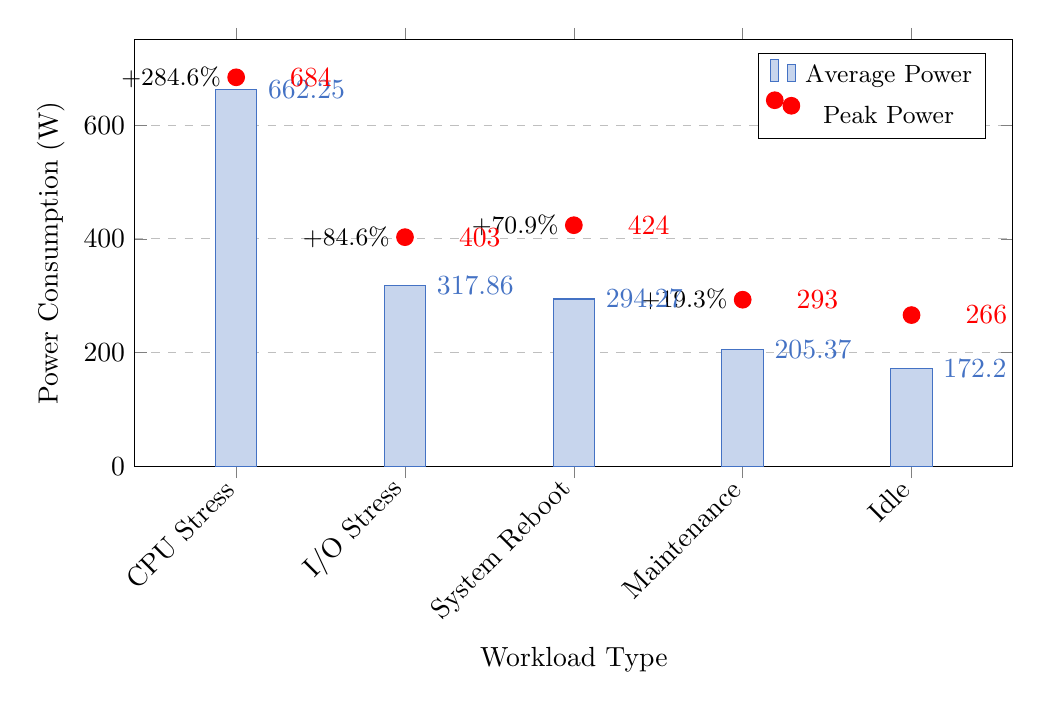
\begin{tikzpicture}
\begin{axis}[
    width=1.05\textwidth,
    height=7cm,
    xlabel={Workload Type},
    ylabel={Power Consumption (W)},
    symbolic x coords={CPU Stress,I/O Stress,System Reboot,Maintenance,Idle},
    xtick=data,
    xticklabel style={rotate=45,anchor=east},
    ybar=5pt,
    bar width=15pt,
    ymin=0,
    ymax=750,
    nodes near coords style={anchor=west, xshift=8pt},
    legend pos=north east,
    legend style={font=\small},
    ymajorgrids=true,
    grid style=dashed,
    clip=false,
    enlarge x limits=0.15
]

% Average power consumption bars with values on the right
\addplot[xblue,fill=xblue!30,
    nodes near coords,
    nodes near coords align={horizontal}
] coordinates {
    (CPU Stress,662.25)
    (I/O Stress,317.86)
    (System Reboot,294.27)
    (Maintenance,205.37)
    (Idle,172.20)
};

% Peak power dots with values on the right
\addplot[xred,only marks,mark=*,mark size=3pt,
    nodes near coords,
    nodes near coords align={horizontal},
    nodes near coords style={anchor=west, xshift=8pt}
] coordinates {
    (CPU Stress,684.0)
    (I/O Stress,403.0)
    (System Reboot,424.0)
    (Maintenance,293.0)
    (Idle,266.0)
};

\legend{Average Power,Peak Power}

% Add percentage increase annotations on the left side
\node[anchor=east, xshift=-2pt] at (axis cs:CPU Stress,684.0) {\small +284.6\%};
\node[anchor=east, xshift=-2pt] at (axis cs:I/O Stress,403.0) {\small +84.6\%};
\node[anchor=east, xshift=-2pt] at (axis cs:System Reboot,424.0) {\small +70.9\%};
\node[anchor=east, xshift=-2pt] at (axis cs:Maintenance,293.0) {\small +19.3\%};

\end{axis}
\end{tikzpicture}
\caption{Comprehensive workload power analysis showing average consumption (bars), peak values (red dots), and percentage increase over idle baseline. The baseline idle power of 172.2W demonstrates significant power variation across different operational states.}
\label{fig:workload-analysis}
\end{figure}

\begin{table}[h]
\caption{Workload Power Consumption Details}
\label{tab:workload-comparison}
\begin{tabular}{@{}lcccc@{}}
\hline
\textbf{Workload} & \textbf{Avg (W)} & \textbf{Peak (W)} & \textbf{Var (W)} & \textbf{kWh} \\
\hline
CPU Stress & 662.25 & 684.0 & ±3.94 & 0.662 \\
I/O Stress & 317.86 & 403.0 & ±52.15 & 0.159 \\
Sys Reboot & 294.27 & 424.0 & ±71.68 & 0.025 \\
Maintenance & 205.37 & 293.0 & ±42.59 & 0.017 \\
Idle State & 172.20 & 266.0 & ±6.82 & 0.172 \\
\hline
\end{tabular}
\end{table}

\subsection{Cost Optimization Potential}
\label{results:optimization}
Analysis of EPEX spot prices during the test period revealed significant optimization opportunities:

\begin{itemize}[noitemsep,topsep=0pt]
    \item Price variation range: -1.685 to 14.168 cent/kWh (230.6\% daily variation from reference price)
    \item Average reference price: 6.874 cent/kWh
    \item Data points for EPEX spot price: 96 (15-minute intervals)
\end{itemize}

Table~\ref{tab:cost-comparison} shows, for each workload, the hypothetical cost if all energy 
had been purchased at the minimum, average, or maximum EPEX spot price observed during the test day. 
The "cost difference" column quantifies the absolute cost reduction possible for each workload 
by shifting all consumption from the most expensive to the cheapest period. Negative costs at the 
minimum price reflect periods of negative electricity pricing, not considering energy grid fees.
\newpage
\begin{table}[h]
    \caption{Workload Cost at Minimum, Average, and Maximum EPEX Spot Price}
    \label{tab:cost-comparison}
    \begin{tabular}{@{}lccccc@{}}
    \hline
    \textbf{Workload} & \textbf{kWh} & \textbf{Min Cost (¢)} & \textbf{Avg Cost (¢)} & \textbf{Max Cost (¢)} & \textbf{Cost Difference (¢)} \\
    \hline
    CPU Stress Test        & 0.662 & -1.12 & 4.55 & 9.38 & 10.50 \\
    I/O Stress Test        & 0.159 & -0.27 & 1.09 & 2.25 & 2.52 \\
    System Reboot          & 0.025 & -0.04 & 0.17 & 0.35 & 0.39 \\
    Maintenance Operations & 0.017 & -0.03 & 0.12 & 0.24 & 0.27 \\
    \hline
    \end{tabular}
    \end{table}

These results demonstrate that intelligent workload scheduling based on real-time electricity 
pricing can lead to substantial cost savings for SMEs operating on-premise server infrastructure. 
The combination of comprehensive energy monitoring and price-aware scheduling provides a practical 
approach to optimizing operational costs while maintaining service quality.

\subsection{Implementation Considerations and Limitations}
\label{results:limitations}
The analysis revealed several key considerations for implementing energy-aware server management:

\begin{itemize}[noitemsep,topsep=0pt]
    \item \textbf{Workload Constraints:}
    \begin{itemize}[noitemsep]
        \item Critical operations cannot always be scheduled optimally
        \item Some workloads require immediate execution regardless of energy costs
        \item Batch processing jobs offer the most flexibility for optimization
    \end{itemize}
    
    \item \textbf{Economic Factors:}
    \begin{itemize}[noitemsep]
        \item Price volatility (230.6\%  daily variation from reference price) enables significant optimization
        \item Benefits scale linearly with server count in SME deployments
        \item Austrian market prices may not reflect other regional patterns
    \end{itemize}
    
    \item \textbf{Technical Limitations:}
    \begin{itemize}[noitemsep]
        \item Single server measurements may not represent diverse hardware configurations
        \item Virtualization overhead affects absolute power measurements
        \item Limited test duration (24 hours) may miss longer-term patterns
    \end{itemize}
\end{itemize}
%Je nach dem in welcher Sprache ihr euer Paper schreiben wollt, benutzt bitte entweder den Deutschen-Titel oder den Englischen (einfach aus- bzw. einkommentieren mittels '%')

%Deutsch
%\section{Schlussfolgerungen und Ausblick}


%Englisch
\section{Conclusion and Future Work}
\label{conclusion:conclusion}
This paper addressed the critical challenge of energy management for SMEs operating on-premise server infrastructure through a cloud-based monitoring and optimization solution. The implementation, detailed in Section~\ref{methodology:prototype} and Appendix~\ref{appendix:github-docs}, successfully integrated IoT-based power monitoring, smart meter data, and real-time electricity pricing to provide actionable insights for cost-effective server operations.

The key contributions of this work include:
\begin{itemize}
    \item A scalable, serverless architecture combining IoT monitoring and real-time pricing data,
    as demonstrated in Section~\ref{methodology:prototype}
    \item Empirical evidence from Section~\ref{results:energy-analysis} demonstrating 
    potential cost savings of up to 10.5 cent per kWh for peak loads (CPU stress test) through intelligent workload scheduling
    \item A practical framework for SMEs to optimize server operations based on energy costs, with implementation details provided in Appendix~\ref{appendix:github-docs}
\end{itemize}

A summary of the experimental results can be found in Section~\ref{results:results}.

While the evaluation demonstrated significant potential for cost optimization (see Section~\ref{results:optimization}), several limitations should be noted:
\begin{itemize}
    \item Single server configuration testing, as described in Section~\ref{methodology:test-infrastructure-setup}
    \item Limited measurement period detailed in Section~\ref{results:limitations}
    \item Focus on Austrian electricity markets (see Appendix~\ref{appendix:strompreis-api})
    \item Manual intervention requirements for workload scheduling
\end{itemize}

Future work should explore:
\begin{itemize}
    \item Machine learning for automated workload scheduling, building on the energy analysis framework (Section~\ref{results:energy-analysis})
    \item Multi-server environment support, extending beyond the current setup (Section~\ref{methodology:test-infrastructure-setup})
    \item Integration with renewable energy sources, complementing the price-based optimization (Section~\ref{results:optimization})
\end{itemize}

The results establish that energy-aware server management can provide substantial benefits for SMEs, creating a foundation for both cost reduction and environmental responsibility. As energy prices continue to rise, such integrated approaches will become increasingly critical for SME competitiveness. The complete implementation and analysis tools are available in the public repository (Appendix~\ref{appendix:github-docs}), enabling further research and practical applications in this domain.
%%
%% The next two lines define the bibliography style to be used, and
%% the bibliography file.
\newpage
\bibliographystyle{ACM-Reference-Format}
\bibliography{section/references}
\label{references:references}

\appendix
\newpage
\section{energyLIVE API Specification}
\label{appendix:energylive-api}

The energyLIVE API, provided by Energie Steiermark, enables the integration of real-time smart meter data into third-party systems, thereby supporting advanced energy management and automation solutions. This interface is designed to facilitate the retrieval of consumption data and system status from smart meters, and can be combined with the smartENERGY electricity price API for dynamic tariff applications such as smartCONTROL.

\subsection{Authentication and Access}

Access to the energyLIVE API requires authentication via an HTTPS header, specifically the \texttt{X-API-KEY}, which must contain a valid key obtained from the customer portal. All requests must be made over secure HTTPS connections to ensure data privacy and integrity.

\subsection{Base URL and Endpoints}
The base URL for the API is:
\begin{quote}
    \url{https://backend.energylive.e-steiermark.com/api/v1/}
\end{quote}
To retrieve the latest measurements from a specific smart meter interface, the following endpoint is used:
\begin{quote}
    \texttt{devices/I-XXXXXXXX-XXXXXXXX/measurements/latest}
\end{quote}
where the interface UID is provided by the customer portal.

\subsection{Data Format and Response Structure}
API responses are returned in JSON format, consisting of an array of measurement objects. Each object contains the following fields:
\begin{itemize}
    \item \textbf{measurement}: Specifies the type of value, typically indicated by an OBIS code for electrical quantities.
    \item \textbf{timestamp}: The time at which the measurement was recorded in the energyLIVE database, represented as a 13-digit Unix timestamp (milliseconds).
    \item \textbf{value}: The measured value, with units such as watt-hours (Wh) for meter readings and watts (W) for instantaneous power.
\end{itemize}

\subsection{Example Request and Response}
A typical request to the API using \texttt{curl} is as follows:
\begin{lstlisting}
curl -X GET -H "X-API-KEY: <your_api_key>" \
"https://backend.energylive.e-steiermark.com/api/v1/devices/I-10082023-01658401/measurements/latest"
\end{lstlisting}

The response is a JSON array, for example:
\begin{lstlisting}
[
  {
    "measurement": "0100010700",
    "timestamp": 1726559995000,
    "value": 138.0
  },
  {
    "measurement": "0100010800",
    "timestamp": 1726559995000,
    "value": 9577201.0
  }
  // ...
]
\end{lstlisting}

\subsection{Use Cases}
The energyLIVE API is suitable for a variety of applications, including the integration of smart meter data into home automation platforms, the development of custom energy monitoring dashboards, and the implementation of dynamic energy management strategies based on real-time consumption and pricing data.

For further details and best practice examples, refer to the official documentation and user community resources provided by Energie Steiermark\footnote{\url{https://www.smartenergy.at/api-schnittstelle-energylive}}.

\newpage
\section{smartENERGY Strompreis API Specification}
\label{appendix:strompreis-api}

The smartENERGY Strompreis API, provided by Energie Steiermark, enables customers to access quarter-hourly electricity price data in real time, facilitating the integration of dynamic pricing information into custom systems and applications. This API supports the automation of energy consumption and the optimization of energy management strategies by providing timely and accurate market price data from the EPEX Spot AT electricity exchange.

\subsection{Authentication and Access}
The Strompreis API is publicly accessible and does not require authentication or special parameters for basic price retrieval. All requests are made via HTTPS to ensure secure data transmission.

\subsection{Base URL and Endpoint}
The base URL for the API is:
\begin{quote}
    \url{https://apis.smartenergy.at/market/v1/price}
\end{quote}
A simple GET request to this endpoint returns the latest available electricity price data.

\subsection{Data Format and Response Structure}
The API returns data in JSON format, with the following structure:
\begin{itemize}
    \item \textbf{tariff}: The tariff identifier, typically set to \texttt{EPEXSPOTAT}.
    \item \textbf{unit}: The unit of the price value, e.g., \texttt{ct/kWh}.
    \item \textbf{interval}: The validity interval of each price entry in minutes (usually 15).
    \item \textbf{data}: An array of objects, each containing:
    \begin{itemize}
        \item \textbf{date}: The local date and time from which the price is valid.
        \item \textbf{value}: The price including 20\% VAT, in decimal format.
    \end{itemize}
\end{itemize}

\subsection{Example Request and Response}
A typical request to the API is as follows:
\begin{lstlisting}
GET https://apis.smartenergy.at/market/v1/price
\end{lstlisting}

The response is a JSON object, for example:
\begin{lstlisting}
{
  "tariff": "EPEXSPOTAT",
  "unit": "ct/kWh",
  "interval": 15,
  "data": [
    {
      "date": "2023-06-23T00:00:00+02:00",
      "value": 12.592
    },
    ...
  ]
}
\end{lstlisting}

\subsection{Use Cases}
The Strompreis API is particularly useful for automating energy consumption in response to real-time price signals, enabling the development of energy management systems that optimize usage patterns according to periods of low electricity prices. It also supports detailed energy monitoring and cost analysis by providing granular, up-to-date market price data.

For further details and best practice examples, refer to the official documentation and user community resources provided by Energie Steiermark\footnote{\url{https://www.smartenergy.at/api-schnittstellen}}.

\newpage
\section{Tasmota Configuration for NOUS A5T Power Strip}
\label{appendix:tasmota-config}

This appendix details the custom Tasmota configuration used for the NOUS A5T power strip, enabling secure integration with AWS IoT and advanced energy monitoring capabilities. The configuration is designed to facilitate reproducibility and ease of deployment for research and practical applications in energy-aware server management.

\subsection{Hardware Overview}
The NOUS A5T power strip features four individually controllable AC outlets, three USB ports, and integrated energy monitoring for voltage, current, and power. The device is based on the ESP8285 microcontroller, which provides 1MB of flash memory and supports custom firmware such as Tasmota.

\subsection{Configuration Purpose and Features}
The custom configuration enables the following key features:
\begin{itemize}
    \item Secure AWS IoT integration with TLS/SSL support
    \item MQTT communication for real-time telemetry
    \item Energy monitoring (voltage, current, power)
    \item Custom device naming and topic structure
    \item Web interface and HTTP API for local management
    \item Rules engine for automation
\end{itemize}

\subsection{Device Template}
The following Tasmota template is used to define the hardware configuration for the NOUS A5T:
\begin{lstlisting}
{
  "NAME": "NOUS A5T",
  "GPIO": [0, 3072, 544, 3104, 0, 259, 0, 0, 225, 226, 224, 0, 35, 4704],
  "FLAG": 1,
  "BASE": 18
}
\end{lstlisting}

\subsection{Custom Firmware Build and Flashing}
To deploy the custom configuration, the following steps should be followed:
\begin{enumerate}
    \item Copy the provided \texttt{user\_config\_override.h} file to the Tasmota source directory:
    \begin{lstlisting}
    copy tasmota-config\user_config_override.h tasmota\tasmota\user_config_override.h
    \end{lstlisting}
    \item Build the custom firmware using PlatformIO:
    \begin{lstlisting}
    cd tasmota
    pio run -e tasmota
    \end{lstlisting}
    \item Flash the firmware to the NOUS A5T device. The built binary is located at \lstinline|tasmota/build_output/firmware/tasmota.bin|. Flashing can be performed via the Tasmota web UI or a serial connection.
\end{enumerate}

\subsection{AWS IoT and MQTT Setup}
After flashing, configure the device for AWS IoT integration using the following Tasmota console command (replace placeholders with your actual AWS IoT endpoint and credentials):
\begin{lstlisting}
BackLog SetOption3 1; SetOption103 1; MqttHost your-endpoint.iot.region.amazonaws.com; MqttPort 443; MqttUser tasmota?x-amz-customauthorizer-name=TasmotaAuth; MqttPassword your-password
\end{lstlisting}

\subsection{Device Information}
\begin{itemize}
    \item \textbf{Name}: Server PowerMeter
    \item \textbf{Topic}: serverpowermeter
    \item \textbf{Firmware}: Custom Tasmota v14.6.0 with AWS IoT support
\end{itemize}

For further details, refer to the configuration file \texttt{user\_config\_override.h} and the project README. This setup enables secure, scalable, and reproducible energy monitoring for research and operational deployments.

\newpage
\section{DynamoDB Cleanup Script: deleteTimestamps.py}
\label{appendix:delete-timestamps}

This appendix documents the Python script \texttt{deleteTimestamps.py}, which is used to clean up the DynamoDB \texttt{SensorData} table by deleting items with timestamps that do not include microseconds. This operation is necessary after migrating to a new timestamp format to ensure data consistency and prevent legacy entries from affecting subsequent analyses.

\subsection{Purpose and Functionality}
The script scans the \texttt{SensorData} table for items whose timestamp attribute (used as the sort key) is exactly 19 characters long, indicating the absence of microseconds. It then interactively deletes these items, using both the partition key and sort key for precise targeting. The script employs exponential backoff to handle DynamoDB throughput limits and provides progress updates during both scanning and deletion phases.

\subsection{Prerequisites}
\begin{itemize}
    \item Python 3.x
    \item \texttt{boto3} and \texttt{botocore} libraries installed (\texttt{pip install boto3 botocore})
    \item AWS credentials configured with permissions to read and delete from the \texttt{SensorData} table
\end{itemize}

\subsection{Usage Instructions}
\begin{enumerate}
    \item Ensure your AWS credentials are set up (e.g., via \texttt{aws configure} or environment variables).
    \item Run the script in a terminal:
    \begin{lstlisting}
    python deleteTimestamps.py
    \end{lstlisting}
    \item Review the summary of items to be deleted and confirm when prompted.
    \item The script will delete the identified items, providing progress updates.
\end{enumerate}

\subsection{Script Listing}
The full source code is provided below for reproducibility:
\begin{lstlisting}[language=Python]
# This script is used to delete items from the SensorData table that have a timestamp 
# without microseconds.
# It is used to clean up the table after the migration to the new format.

import boto3
import time
from botocore.exceptions import ClientError

# Initialize DynamoDB
dynamodb = boto3.resource('dynamodb')
table = dynamodb.Table('SensorData')

print("Checking table schema...")

# Get table description to find primary key
table_description = table.meta.client.describe_table(TableName='SensorData')
key_schema = table_description['Table']['KeySchema']

print("Table key schema:")
for key in key_schema:
    print(f"  {key['AttributeName']} ({key['KeyType']})")

# Find the partition key and sort key
partition_key_name = None
sort_key_name = None
for key in key_schema:
    if key['KeyType'] == 'HASH':  # Partition key
        partition_key_name = key['AttributeName']
    elif key['KeyType'] == 'RANGE':  # Sort key
        sort_key_name = key['AttributeName']

if not partition_key_name or not sort_key_name:
    print("ERROR: Could not find partition key or sort key")
    exit(1)

print(f"Partition key: {partition_key_name}")
print(f"Sort key: {sort_key_name}")

print("Scanning DynamoDB table...")

# Count items without microseconds
count_without_microseconds = 0
items_to_delete = []
total_scanned = 0

def scan_with_retry(exclusive_start_key=None):
    """Scan with exponential backoff for throughput exceptions"""
    max_retries = 5
    base_delay = 1
    
    for attempt in range(max_retries):
        try:
            if exclusive_start_key:
                response = table.scan(
                    ExclusiveStartKey=exclusive_start_key,
                    ProjectionExpression='#pk, #sk',
                    ExpressionAttributeNames={
                        '#pk': partition_key_name, 
                        '#sk': sort_key_name
                    }
                )
            else:
                response = table.scan(
                    ProjectionExpression='#pk, #sk',
                    ExpressionAttributeNames={
                        '#pk': partition_key_name, 
                        '#sk': sort_key_name
                    }
                )
            return response
        except ClientError as e:
            if e.response['Error']['Code'] == 'ProvisionedThroughputExceededException':
                if attempt < max_retries - 1:
                    delay = base_delay * (2 ** attempt)  # Exponential backoff
                    print(f"Throughput exceeded, waiting {delay} seconds...")
                    time.sleep(delay)
                else:
                    raise
            else:
                raise

# Scan with pagination to get all items
try:
    response = scan_with_retry()
    
    # Process first batch
    for item in response['Items']:
        total_scanned += 1
        timestamp = item[sort_key_name]  # Use sort key name
        if len(timestamp) == 19:  # No microseconds
            count_without_microseconds += 1
            # Use both partition key and sort key for deletion
            delete_key = {
                partition_key_name: item[partition_key_name],
                sort_key_name: item[sort_key_name]
            }
            items_to_delete.append(delete_key)
    
    # Continue scanning while there are more items
    while 'LastEvaluatedKey' in response:
        print(f"Scanned {total_scanned} items so far...")
        time.sleep(0.1)  # Small delay between scans
        
        response = scan_with_retry(response['LastEvaluatedKey'])
        
        for item in response['Items']:
            total_scanned += 1
            timestamp = item[sort_key_name]  # Use sort key name
            if len(timestamp) == 19:  # No microseconds
                count_without_microseconds += 1
                # Use both partition key and sort key for deletion
                delete_key = {
                    partition_key_name: item[partition_key_name],
                    sort_key_name: item[sort_key_name]
                }
                items_to_delete.append(delete_key)

except ClientError as e:
    if e.response['Error']['Code'] == 'ProvisionedThroughputExceededException':
        print("ERROR: DynamoDB throughput exceeded. Consider:")
        print("1. Increasing provisioned throughput")
        print("2. Running this script during off-peak hours")
        print("3. Using on-demand billing mode")
    else:
        print(f"ERROR: {e.response['Error']['Message']}")
    exit(1)

print(f"Total items scanned: {total_scanned}")
print(f"Found {count_without_microseconds} items without microseconds")

if count_without_microseconds > 0:
    # Show first few items to delete
    print("First 5 items to delete:")
    for item in items_to_delete[:5]:
        print(f"  {item}")
    
    # Ask for confirmation
    confirm = input("Do you want to delete these items? (yes/no): ")
    if confirm.lower() == 'yes':
        # Delete items with rate limiting
        deleted_count = 0
        for item in items_to_delete:
            try:
                table.delete_item(Key=item)
                deleted_count += 1
                if deleted_count % 50 == 0:  # Progress update every 50 items
                    print(f"Deleted {deleted_count} items...")
                    time.sleep(0.1)  # Small delay
            except ClientError as e:
                if e.response['Error']['Code'] == 'ProvisionedThroughputExceededException':
                    print(f"Throughput exceeded while deleting. Stopped at {deleted_count} items.")
                    break
                else:
                    print(f"Error deleting item: {e.response['Error']['Message']}")
        print(f"Successfully deleted {deleted_count} items")
    else:
        print("Deletion cancelled")
else:
    print("No items found without microseconds")
\end{lstlisting}

\newpage
\section{GitHub Repository and Documentation}
\label{appendix:github-docs}

This appendix provides permanent references to the project's GitHub repository and its core documentation. The repository contains all source code, configuration files, and documentation required to replicate the research and implementation described in this paper.

\subsection{Repository Information}
\begin{itemize}
    \item \textbf{Repository URL}: \url{https://github.com/papers-mcce/energyops}
    \item \textbf{Main Branch}: \texttt{main}
    \item \textbf{Documentation Branch}: \texttt{final-paper}
\end{itemize}

\subsection{Core Documentation Structure}
The repository's documentation is organized hierarchically, with the main README.md serving as the entry point. Key documentation components include:

\subsubsection{Main Project Documentation}
The primary README.md (\url{https://github.com/papers-mcce/energyops/blob/main/README.md}) provides:
\begin{itemize}
    \item Project overview and objectives
    \item Complete directory structure
    \item Deployment instructions
    \item Configuration guides
    \item Replication procedures
\end{itemize}

\subsubsection{Component-Specific Documentation}
\begin{enumerate}
    \item \textbf{Terraform Infrastructure} \\
    \url{https://github.com/papers-mcce/energyops/blob/main/Deployment/terraform/README.md}
    \begin{itemize}
        \item AWS resource specifications
        \item Deployment procedures
        \item Security configurations
        \item Infrastructure diagrams
    \end{itemize}

    \item \textbf{Energy Analysis Tools} \\
    \label{appendix:energy-analysis}
    \url{https://github.com/papers-mcce/energyops/blob/main/Deployment/Energy-Analysis/README_energy_analysis.md}
    \begin{itemize}
        \item Data collection scripts
        \item Analysis methodologies
        \item Visualization tools
        \item Result interpretation guides
    \end{itemize}

    \item \textbf{Tasmota Configuration} \\
    \url{https://github.com/papers-mcce/energyops/blob/main/tasmota-config/README.md}
    \begin{itemize}
        \item Device setup instructions
        \item Custom firmware configuration
        \item AWS IoT integration steps
        \item Troubleshooting guides
    \end{itemize}

    \item \textbf{HTML Presentation} \\
    \url{https://github.com/papers-mcce/energyops/blob/main/html-presentation-project/README.md}
    \begin{itemize}
        \item Interactive visualization setup
        \item Deployment instructions
        \item Customization options
        \item Browser compatibility notes
    \end{itemize}
\end{enumerate}

\subsection{Cross-References and Dependencies}
The documentation maintains internal cross-references using LaTeX labels. Key references include:
\begin{itemize}
    \item Energy Analysis (Section~\ref{appendix:energylive-api})
    \item Price API Documentation (Section~\ref{appendix:strompreis-api})
    \item Device Configuration (Section~\ref{appendix:tasmota-config})
    \item Database Management (Section~\ref{appendix:delete-timestamps})
\end{itemize}

\subsection{Version Control and Updates}
The documentation is maintained under version control, with updates tracked through Git commits and pull requests. Major changes are documented in the repository's release notes and change logs.

For the most current version of any documentation component, refer to the repository URLs provided above. All links are permanent and reference specific commits to ensure reproducibility of the research implementation.

\section*{Reproducibility Note}
All scripts, infrastructure code, and setup guides referenced in this paper are included in the project materials to support full reproducibility of the research and experiments described.


\end{document}
\endinput
%%
%% End of file `sample-acmlarge.tex'.
